\documentclass[12pt, a4paper, twoside]{report}
\usepackage[utf8]{inputenc}
\usepackage[T1]{fontenc}      
\usepackage[francais]{babel}
\usepackage{amsmath}
\usepackage{amsfonts}
\usepackage{amssymb}
\usepackage{graphicx}
\usepackage{hyperref}
\usepackage{caption}
\usepackage{eurosym}
\usepackage{wrapfig}
\usepackage{rotating}
\usepackage{float}
\usepackage{fancyhdr, emptypage}
\usepackage[pass]{geometry}       %% showframe just for demo
\usepackage{hyperref}
\hypersetup{
	colorlinks = false,
	pdfborder={0 0 0},
}
\usepackage{titlesec}
\usepackage{array,tabularx}

\usepackage{float}
\titleformat{\chapter}[display]   
{\normalfont\huge\bfseries}{\chaptertitlename\ \thechapter}{20pt}{\Huge}   
\titlespacing*{\chapter}{0pt}{-50pt}{40pt}

\pagestyle{fancy}
\fancyhf{}
\fancyfoot[CE,CO]{\leftmark}
\fancyfoot[LE,RO]{\thepage}
\renewcommand{\footrulewidth}{1pt}
\renewcommand{\headrulewidth}{0pt}
\usepackage{array, multirow}
\usepackage[usenames,dvipsnames,svgnames,table]{xcolor}
\newcolumntype{M}[1]{>{\centering\arraybackslash}m{#1}}
\renewcommand{\baselinestretch}{1.5}

\newcommand{\mychapter}[2]{
	\setcounter{chapter}{#1}
	\setcounter{section}{0}
	\chapter*{#2}
	\addcontentsline{toc}{chapter}{#2}
}

\newcommand{\HRule}{\rule{\linewidth}{0.5mm}}

\author{Aline CHETTA \\
	Master 1 Bio-Informatique et Bio-Statistique
	Nantes
	France}
\date{9 mai 2016}
\title{Rapport de stage}
\begin{document}
	\newgeometry{hmarginratio=1:1}    %% make layout symmetric
	\begin{titlepage}
		\center
		
		\textsc{\huge Université de Nantes}\\[1.5cm]
		{\scshape\LARGE Rapport de stage\par}
		\rule[0.5ex]{\linewidth}{2pt}\vspace*{-\baselineskip}\vspace*{3.2pt}
		\rule[0.5ex]{\linewidth}{1pt}\\[\baselineskip]
		{ \huge \bfseries Développement Web et Solution e-commerce Magento}\\[0.4cm]
		\rule[0.5ex]{\linewidth}{2pt}\vspace*{-\baselineskip}\vspace*{3.2pt}
		\rule[0.5ex]{\linewidth}{1pt}\\[\baselineskip]
		
		
		{\Large Aline \scshape \textsc{Chetta}\par}
		{\large Master 1 Bio-Informatique et Bio-Statistique\par}
		{\large \today\par}
		
		\vspace{3.5cm}
		
		\begin{minipage}{0.45\textwidth}
			\begin{flushleft} \Large
				\emph{Maître de stage :}\\
				Thibault \textsc{Vacher}\\
				
\includegraphics[width=0.75\textwidth]{Images/Smile.png}\par\vspace{1cm}
			\end{flushleft}
		\end{minipage}
		\begin{minipage}{0.45\textwidth}
			\begin{flushright} \Large
				\emph{Tuteur de stage :}\\
				Bernard \textsc{Offmann}
				
\includegraphics[width=0.75\textwidth]{Images/logo-iut.png}\par\vspace{1cm}
			\end{flushright}
		\end{minipage}\\[1.5cm]
		% Bottom of the page
		\vfill
	\end{titlepage}
	
	\restoregeometry              %% restore the layout
	
	\newpage\null\thispagestyle{empty}\newpage
	
\mychapter{-3}{Remerciements}

Je remercie tout d'abord la société Smile pour l'opportunité qu'elle m'a donnée pour effectuer ce stage. \\

Je tiens à remercier mon maître de stage, Monsieur Thibault \textsc{Vacher} pour m'avoir accueilli dans le service e-commerce. \\

Je remercie aussi Madame Julie \textsc{Clabault} pour avoir pris le temps de m'expliquer l'organisation et les différentes procédures de travail et Monsieur Dorian \textsc{Brun} pour sa patience et son expertise lors des difficultés rencontrés dans mon travail. \\

Enfin, je remercie les différentes équipes pour leur bonne humeur et leur accueil.


\newpage\null\thispagestyle{empty}\newpage

\setcounter{tocdepth}{2}
\begingroup\makeatletter
\def\@makeschapterhead#1{%
	{\parindent \z@ \raggedright
		\normalfont
		\interlinepenalty\@M
		\Huge \bfseries  #1\par\nobreak
}}\makeatother
\tableofcontents
\endgroup




\mychapter{-4}{Résumé}

J’ai effectué mon stage au sein la société Smile qui m'a permis de participer aux développements web de plusieurs sites e-commerce. \vspace{0.1cm}

Au cours de ce stage, j'ai intégré plusieurs équipes de développement. Chaque équipe est composé d'un(e) chef de projet et d'un(e) \textit{lead developper}. Le chef de projet répartit le travail entre chaque développeur selon leur spécialisation et leur aptitude. Le \textit{lead developer} a en outre pour tâche de valider ou non les modifications apportées et d'assurer les livraisons du code. \\
Il existe des procédures propres à chaque projet. Si ces dernières ne sont pas respectées, les évolutions apportées ne seront jamais prise en compte. De plus, lorsqu'un développeur contribue à un projet, il se doit de respecter certaines règles de bonnes pratique, les principes de base pour la programmation orientée objet (SOLID) et la philosophie « Une fonction fait une seule chose et elle le fait bien ». \vspace{0.1cm}

J'ai eu l'opportunité de travailler avec la solution Magento 1 pour les projets Wacama (Camif \& Matelsom) et Bocage. J'ai notamment travaillé sur la partie TMA du projet. Cela signifie que mes principaux objectifs étaient la correction des anomalies, d'assurer un rôle de support pour le client et d'intégrer de nouvelles fonctionnalités. \\
Enfin, le dernier projet auquel j'ai participé est le nouveau site de Speed Burger. Ce projet est en cours de validation des spécifications donc tout reste encore à faire. Ma principale mission pour ce projet est de développer des modules propres à l'application sous Magento 2. \vspace{0.1cm}

\textbf{Mots-clé :} Magento, Développement Web, Open Source, Git, Redmine, Smile

\mychapter{-3}{Abstract}

I did my internship at a company named Smile which made me participate in the developments of several e-commerce websites. \vspace{0.1cm}

During this course, I was part of several development teams. Each team is composed of a project leader and a lead developer. The project manager dispatches the work between each developer according to their specialization and their aptitudes. The lead developer also has the task to validate or not the modifications made and allow to put our code live into production. \\
There are procedures specific to each project. If they are not respected the changes brought will never be taken into account. In addition, when a developer contributes to a project, he must respect a few "good practices" rules, the SOLID's principles and the rule : "A function does one thing and does it well.". \vspace{0.1cm}

I had the opportunity to work with the Magento 1 framework for the Wacama projects (Camif \& Matelsom) and Bocage. I worked on the TMA part of the project. My main focus was to correct anomalies, ensuring support for the client and integrating new functionalities. \\

Finally, the last project I participated in was Speed Burger. This project is in the process of validating specifications so everything still has to be done. My main mission for this project is to develop specific modules for the application now build with Magento 2. \vspace{0.1cm}

\textbf{Keywords:} Magento, Developpement Web, Open Source, Git, Redmine, Smile

\mychapter{-2}{Introduction}

Dans le cadre de ma formation en Master I Bio-Informatique à l'université de Nantes, un stage de minimum 2 mois est à réaliser afin de valider son année de formation. Ce stage a pour objectif d'acquérir une expérience professionnelle, de mettre en application les connaissances acquises au cours de l'année et de monter en compétence au travers de projets professionnels. \\

Pour ma part, j'effectue ce stage au sein de la société Smile depuis le 27 Mars jusqu'au 18 Août 2017. Cette société est connue pour être le premier intégrateur de solutions web open-source. Ils ont pour clients de nombreuses sociétés françaises et européennes. L’agence de Nantes est composée d’une cinquantaine de collaborateurs et elle est principalement axée sur le développement e-commerce avec la solution Magento et sur le développement web avec le framework Symfony. \\

Le sujet de mon stage est de participer au développement de différents projets e-commerce en cours et ayant pour point commun l'utilisation du langage PHP et de la plateforme Magento. Le but est ici de corriger des anomalies détectées, d'intégrer les nouvelles fonctionnalités et d’assurer un rôle de support pour chaque demande ou problème rencontré par le client. \\

Afin d’intégrer au plus tôt l’équipe de développement, Smile propose d’effectuer une formation générale au début du stage sur l’environnement de base que rencontre un développeur au sein de la société. De plus, afin de me préparer à mon principal projet de développement (Speed Burger), j’ai également effectué une formation Magento 2.

\mychapter{-1}{Abréviations}
\begin{itemize}
	\item \textbf{\textsc{css}} : Cascading Style Sheets : feuilles de styles en cascade utilisées pour définir un ensemble de règles qui régissent l'apparence d'éléments dans une page \textsc{html}.
	\item \textbf{\textsc{html}} : HyperText Markup Language : format permettant de structurer une page web.
	\item \textbf{\textsc{tma}} : Tierce Maintenance Applicative : externalisation de la maintenance d'une application d'une entreprise auprès d'un prestataire.
	\item \textbf{\textsc{xml}} : Extensible Markup Language : langage de balise permettant de décrire le contenu d'une page. 
	\item \textbf{\textsc{sass}} : Sassy CSS est un langage de programmation capable d’imbriquer des règles de style.
	\item \textbf{\textsc{poo}} : Programmation Orienté Objet.
	\item \textbf{\textsc{mvc}} : Modèle d'architecture de dossier décomposant le code selon le Modèle, la Vue et le Contrôleur.
	\item \textbf{\textsc{psr}} : PHP Standards Recommandation.
	
\end{itemize}

\mychapter{0}{Glossaire}
\begin{itemize}
	\item \textbf{Framework} : Ensemble de composants et d'outils formant les fondation de l'application.
	\item \textbf{\textit{Merge request}} : Requête envoyée au \textit{lead developer} afin d'appliquer des changements de code d'une branche à une autre.
	\item \textbf{\textit{From scratch}} : Refonte complet d'un projet. Aucune base n'est récupérée du projet courant.
	\item \textbf{Pop-in} : fenêtres qui ne s'ouvrent qu'à l'intérieur d'une page web, contrairement aux pop-ups.
\end{itemize}
\thispagestyle{empty}

\newpage\null\thispagestyle{empty}\newpage

\chapter{Sujet du Stage}

\section{Présentation du Sujet}

Le principal but de ce stage est de participer à l'élaboration et au maintien d'un site e-commerce. Contrairement aux idées reçues, un site e-commerce n'est pas un site vitrine. Il répond notamment à deux comportements. Le premier est la possibilité pour un consommateur d'effectuer une commande et d'en avoir un suivi. Le second est d'effectuer directement sur le site un achat de produits ou de services par paiement sécurisé. L'atout d'un site e-commerce pour le marchand est de pouvoir accéder à une interface d'administration lui permettant de modifier directement certains paramètres de ces produits. \\ 

À la différence d'une application web standard, un site e-commerce doit être en mesure de supporter un important catalogue de produits mais surtout d'être ergonomique, sécurisé et simple d'utilisation pour l'utilisateur. Un site dynamique et correctement référencé est un atout indéniable au succès commercial du marchand. De plus, à l'ère du numérique, les performances d'un site e-commerce doivent être suffisante sur tous les types de surfaces. \\

Pour se démarquer et assurer le fonctionnement d'un site e-commerce, nombreuses sont les entreprises faisant appel à des prestataires. Smile est une société connue de l'e-commerce grâce à son partenariat avec Magento. Cette solution open-source se compose du site e-commerce accessible à tous les utilisateurs une fois mis en production et d'une partie \textit{back-office} permettant à l'entreprise de manager ses produits et de connaître le comportement de ses clients par des données statistiques. Le développement sous Magento est réalisé en orienté objet (POO). De plus, il respecte un modèle MVC (Modèle Vue Constructeur) avancé permettant ainsi de classer les dossiers par fonctionnalité et donc de séparer les éléments du \textit{front} et du \textit{back-end} afin de faciliter le développement. Il dispose également de nombreuses fonctionnalités natives qui peuvent être aisément surchargées, c'est à dire étendues pour mettre en place des fonctionnalités sur-mesure demandées par le client\footnote{La notion de client désigne l'entreprise pour laquelle la conception d'un site e-commerce est réalisée, cela sera le cas tout au long de ce rapport de stage.}.


\section{Présentation des Projets}

 Actuellement, de nombreux projets sont en cours de réalisations au sein de Smile. La principale mission qui m'a été attribué est de participer au développement du projet Speed Burger. Ce projet consiste à effectuer une refonte complète (from scratch) du site. Néanmoins puisque les spécifications n'étaient pas encore signées à mon arrivée, j'ai également participé aux projets Wacama (Camif et Matelsom) et Bocage. \\
 
 \begin{table}[H]
 	\centering
 	\resizebox{\textwidth}{!}{%
 	\begin{tabular}{|c|c|} 
 		\hline
 		\rowcolor[HTML]{D5D5D5} 
 		\textbf{Projets} & \textbf{Principaux Objectifs} \\ 
 		\hline
 		\rowcolor[HTML]{FFFFFF} 
 		Camif            & Refonte, Création \textit{API} Panier et Tunnel de commande, TMA, SEO \\ 
 		\hline
 		Matelsom         & TMA \\ 
 		\hline
 		\rowcolor[HTML]{FFFFFF} 
 		Bocage           & TMA, Mise en place d'une version mobile \\ 
 		\hline
 		Speed Burger     & Refonte \textit{from scratch}, Mise en place pour le lot 1\footnote{Première livraison de l'application au client} du catalogue de produits, Gestion des flux.\\ 
 		\hline
 	\end{tabular}}
 \caption{ Tableau récapitulatif des objectifs principaux pour chaque projet auquel j'ai participé.}
 \end{table}

Le tableau ci-dessus montre la grande variété de tâches et d'organisation à effectuer tout le long d'un projet. Chacun des projets est organisé de façon unique (TMA, forfait, régie) selon les différentes missions et selon le cahier des charges établi entre le client, le chef de projet, ainsi que l'équipe commerciale. 


\section{Objectif du Stage}

L'objectif premier de ce stage est de monter en compétence notamment sur Magento mais aussi sur l'environnement de développement. Pour m'aider, la société Smile m'a permis de réaliser deux formations de 4 jours. La première est la \textit{Smile Academy} centrée sur les outils de développement principalement utilisé au sein de la société et la seconde était portée sur la solution Magento 2 ainsi que ses bonnes pratiques. \\ 

Pour les projets Wacama et Bocage, ma mission est d'assurer une partie des Tierces Maintenances Applicatives (TMA). La maintenance applicative consiste à assurer le bon fonctionnement d'une application, c'est-à-dire de corriger des anomalies, d'adapter le comportement d'un module selon l'utilisation réelle d'un consommateur et d'effectuer des améliorations suite à l'évolution de l'application. De plus sur le projet Camif, j'ai eu pour autre missions de contribuer au SEO du site web. Pour Speed Burger, la mission est principalement de participer au développement des modules sous Magento\footnote{Lorsque ce rapport sera rendu, je n'aurai travaillé qu'une semaine sur ce projet.} et de respecter les règles de bonne pratiques lors la création des différents modules. 

\chapter{Analyse de l'existant}

\section{Outils relatifs aux projets}

Chaque projet est mené sous la direction d'un directeur technique (\textit{lead developer}). Ce dernier se charge d'initier le projet en créant une un environnement de développement isolé permettant l'installation de la solution Magento, de modules tiers et d'éléments de configuration du projet. Cet environnement doit être semblable à celui de l'hébergeur de l'application. Smile utilise un système de conteneurs LXC , qui n'est pas une machine virtuelle, mais permet de créer un environnement neutre et propre, non influencé par les projets extérieurs. Ainsi lors de la migration en production, aucun conflit n'est à prévoir avec l'environnement du serveur. \\

Le deuxième outil essentiel est Git. Ce dernier est un logiciel de gestion de versionnage. Chaque projet dispose de son dépôt distant, privé, géré par l'application GitLab. Ainsi chaque collaborateur doit être en mesure d'accéder à ce dépôt et d'y envoyer leur contribution.  \\

Lors de la création d'un tel projet, il est conseillé de construire trois branches. Chaque branche correspond à une version alternative d'un projet. En simplifiant, disons qu'il s'agit d'un état différent du dépôt mais ayant une même origine (Schéma explicatif). La branche par défaut \textit{master} correspond à l'application présente en production. La seconde est la branche \textit{recette}. C'est au sein de cette branche que le client peut constater les modifications, effectuer des retours ou valider les changements opérés. La dernière branche est la branche \textit{preprod}. Elle correspond à la branche de développement et c'est ici où est validé le travail achevé de chaque développeur par le \textit{lead developer}. Ainsi lorsqu'une amélioration ou une correction du code est effectuée sur la branche préprod, elle est déployée sur l'environnement de recette ou de production grâce à l'outil Ansible. \\

\begin{figure}[H]
	\centerline{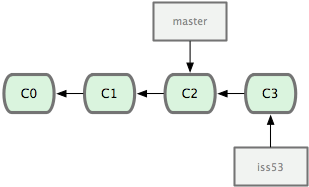
\includegraphics[scale=0.5]{Images/image.png}}
	\caption{Figure montrant l'avancement de la branche iss53 depuis la branche master.}
\end{figure}

Pour répartir le travail entre les développeurs, le chef de projet crée des tickets (tâches à effectuer selon les demandes du client) sur l'application Redmine et les attribue aux développeurs du projet. Lorsque un ticket est accompli, il doit être validé par le \textit{lead developer} puis par le chef de projet. Ensuite, si son retour est positif, les changements seront inclus lors de la prochaine migration en recette ou en production. Un wiki est intégré à Redmine et permet d'expliquer la démarche à suivre pour paramétrer certain éléments du projet mais également de connaître les modules présents et d'accéder aux différentes URL du projet (site web / \textit{back-office} / git). \\

Enfin, concernant l'architecture des serveurs de production, ils sont généralement organisés de la façon suivante.

	\makebox[\textwidth]{Nginx $\rightarrow$ Varnish $\rightarrow$ Apache} \par
	
Lorsqu'un utilisateur rentre le chemin du site e-commerce, la requête HTTPS est traitée par Nginx, qui renvoie la requête HTTP à l'application Varnish. Cette dernière a pour principale fonction de gérer le cache de l'application. En effet, lorsque l'utilisateur demande une page, Varnish vérifie si les données sont stockées dans son cache. Si c'est le cas, il affiche directement la page sinon il demande de générer la page au serveur Apache en lui fournissant les informations nécessaires.
	

\section{Langages relatifs aux projets}

La solution Magento est construite avec le langage PHP et son interface est basée sur les technologies CSS et JavaScript. \\

Afin de simplifier et améliorer la visibilité du code, des extensions et des modules complémentaires ont été installés par l'intermédiaire de l'outil composer (gestionnaire de bibliothèques PHP) ainsi que Gulp. Ce dernier permet d'automatiser l'ensemble des tâches liées au CSS. Par exemple, il est possible de compiler des fichiers SASS (.SCSS) en CSS. Le SASS contrairement au CSS est un vrai langage de programmation permettant la création de variables et surtout la possibilité d’imbriquer des règles de style. Concernant le Javascript, les deux frameworks utilisés personnellement sont jQuery et Prototype, qui sont présent nativement dans Magento. Comme pour le CSS, un autre outil du nom de Grunt permet la compilation automatique du JS.


\section{Wacama}

Ce projet regroupe la mise en place de deux sites e-commerce sous Magento gérés jusqu'à présent par un seul \textit{back-office}. Ainsi, ces applications possèdent des composants en commun. Smile collabore avec ce groupe depuis plus de 5 ans. De nombreux modules tiers ont été mis en place. Une liste des composants utilisés lors de mon stage est présentée ci-dessous. \\

\begin{description}
	\item[Fredhopper] Ce service permet d'améliorer le temps de réponse lors d'une recherche de produits. Il est également capable de créer des facettes (critères de sélection) et de trier les produits dans une catégorie. \\
	
	\item[Akaneo] Cette solution est un PIM (Product Information Management). Elle permet la gestion du catalogue de produit en un seul et même point. En autre terme, il s'interface entre chaque système tiers afin de centraliser l'information et ainsi de contrôler la qualité des données et d'exporter ces données aisément entre chaque module (exemple : références différentes des produits ente MySQL et FredHopper). \\
	
	\item[Mirakl] C'est un outil de gestion de \textit{marketplace}. Il permet aux entreprises d'étendre leur offre de produits en incluant d'autres vendeurs. \\
\end{description}

\section{Bocage}

Au sein de ce projet où Magento a été mis en place, je n'ai exploité qu'un seul outil supplémentaire. Il s'agit de ngrok. Sa fonctionnalité est de créer un tunnel sécurisé depuis le réseau extérieur jusqu'à sa machine locale. Dès lors, il est possible de tester son application en cours de développement sur mobile ou d'autoriser l'accès à son travail à un autre collaborateur.

\section{Speed Burger}

Contrairement aux deux autre projets, ce site e-commerce est développé sous Magento 2. Cette nouvelle version a subi énormément de changements. Ses nouvelles améliorations permettent de mieux supporter les pointes d'utilisation du site par les consommateurs, de rendre plus rapide les temps de chargement et de supporter un plus grand nombre de produits. Un thème \textit{responsive} de base est également proposé. Mais surtout une refonte de l'interface d'administration a été réalisé, elle est désormais moderne et intuitive. \\ 

Au niveau du code, Magento 2 respecte les normes d'écritures du PSR (PHP Standards Recommandation). De plus, puisque la solution est désormais installée par Composer, l'architecture des dossiers a été modifiée. L'organisation des dossiers au sein d'un module de l'application est plus strict. Cela permet d'augmenter la compréhension de l'organisation du code mais surtout de respecter le modèle MVC. \\

Comme dit précédemment dans ce rapport, le projet vient de débuter et toutes les spécifications ne sont pas encore validée par l'entreprise. Par conséquent, aucun autre module tiers n'a été encore été installé. Au stade actuel, le but est de mettre en place le catalogue de produits, de gérer les flux entre les ERPs et la caisse et permettre la gestion des produits et des services dans le \textit{back-office}.
% #DEFINE ERP;

\chapter{Développement}

\section{Organisation du travail}

\subsection{Outil de développement}

La solution Magento dispose d'une architecture complexe. Afin de faciliter le développement, Smile utilise l'IDE (Environnement de développement) PhpStorm. Cet éditeur permet d'avoir une vue globale sur l'ensemble des fichiers du projet et de visualiser leur type. Il dispose d'une auto-complétion puissante, est capable de prévenir des erreurs syntaxique en temps réel et permet une navigation rapide entre les différents fichiers. Cette dernière fonctionnalité est très utile pour vérifier quelle classe est appelée et à quoi correspond telle ou telle variable. De plus, il détecte automatiquement si un dépôt Git est configuré et synchronise les modifications en comparant avec l'état précédent de la branche. \\

Avec cet IDE, il est également possible d'ajouter des modules notamment celui pour Magento 2. Il permet notamment d'améliorer l'auto-complétion. Il est toutefois nécessaire de prendre du temps pour le configurer afin que PhpStorm puisse comprendre le langage XML. \\

Enfin, un outil indispensable pour le débogage PHP est XDebug. Ce débogueur permet de simplifier et de faciliter la phase de débogue. Si la configuration est réalisée correctement, cet outil est détecté par PhpStorm et il est dès lors possible de l'utiliser directement. Une fois activé, il suffit de mettre un pointeur sur la fonction à déboguer et de recharger la page pour visionner directement sur l'IDE les informations sur l'état des variables au moment t et connaître la pile des appels de méthodes. Plusieurs fonctionnalités sont alors accessibles notamment le parcours de la méthode pas à pas et l'accès à l'inspecteur qui permet de connaître l'état présent d'une variable ciblée.

\subsection{Traitement d'un ticket}

Pour rappel, le chef de projet attribue un ticket sur Redmine à un développeur. Un ticket est composé d'un identifiant et de l'ordre de mission. \\

Le premier réflexe à avoir est de changer le statut du ticket sur Eedmine de \textit{nouveau} à \textit{en cours}. \\

Il existe deux types de tickets généralement les anomalies (\textit{Fix}) et les améliorations (\textit{Feat}) en Tierce Maintenance Applicative. Lors d'un travail en TMA, il est nécessaire de créer une branche par ticket. La procédure à suivre est expliquée ci-dessous :
\begin{enumerate}
	\item Création d'une branche à partir de la branche \textit{preprod} ayant la cette nomenclature :
	
		\makebox[\textwidth]{\texttt{\$ git checkout -b Type-Identifiant}}
		
	\item Développement et commit en anglais. Un commit est une commande permettant d'enregistrer son travail. Il doit être sous la forme : 
	
		\makebox[\textwidth]{\texttt{\$ git commit -m "Type \#Identifiant : Rapide description"}}
		
	\item Création de la merge request en assignant le \textit{Lead developer} pour validation.\\
		
\end{enumerate}

Lors un développement de module, une branche par développeur est suffisante. Néanmoins, il est toujours nécessaire de suivre les règles de commit. \\

Dès la merge request effectuée, le statut du ticket sur Redmine doit encore être modifié en « \textit{A livrer en recette interne} ».  \\

Si l'ensemble de ces règles n'est pas respecté, le ticket ne sera pas validé. Le but de cette procédure est de simplifier le travail du \textit{Lead developer} mais surtout de garder un historique compréhensible des différentes tâches réalisées sur la branche \textit{preprod} pour enfin livrer le code validé par les clients.

\subsection{Imputation}

Pour facturer au client le temps de travail de chaque collaborateur d'un projet, deux systèmes de calcul sont mise en place. \\

- Dans Redmine, le temps en heure de travail doit être renseigné pour chaque ticket. Si un ticket a un temps estimé, il est nécessaire de préciser si il y a eu dépassement ou si dépassement il y aura. Cela permet au chef de projet de prendre des mesures afin de respecter au mieux le cahier des charges.

- Un outil interne \textit{Gescom} permet d'imputer son temps de travail par jour selon le projet travaillé en renseignant les contributions effectuées. \\

Il est important de bien renseigner son temps sur Redmine et de prévenir le chef de projet si le temps nécessaire à la tâche est insuffisant car le client y a accès et peut donc demander des comptes s'il s'aperçoit d'anomalies ou de temps de dépassement trop fréquents. Il ne faut donc pas estimer le nombre d'heures d'un projet à la baisse pour faire diminuer les coûts.


\section{Environnement technique}

\subsection{Wacama}

Pour apprendre, il n'y a rien de mieux que la pratique. Dès la première semaine, j'ai commencé à traiter des tickets concernant la TMA. \\

Dans un premier temps, j'ai travaillé sur des tickets simples consistant à faire des modifications en CSS et de corriger des anomalies faciles à traiter. J'ai notamment entre autres développé une \textit{pop-in} permettant l'affichage d'une description pour les frais de traitement dans le panier et dans le tunnel de commande. Comme ce projet concerne deux sites web différents, les demandes d'améliorations ou de correctifs sont généralement réalisées sur les deux. J'ai réalisé ce ticket en début de stage en mettant en place une fonction jQuery et un peu de SASS. Toutefois, lors de la refonte du site Camif et de la création de l'API Panier, j'ai dû de nouveau retravailler sur ce ticket , d'où l'importance de la TMA. De plus, avec l'expérience gagnée, j'ai pu simplifier le code, notamment la partie SASS. \\

De plus, j'ai également travaillé sur des modules spécifiques. J'ai notamment corrigé un bug entraînant une erreur dans le module \textit{commander} (permettant au client d'avoir des informations lorsqu'un consommateur est en train d'effectuer un achat) et j'ai aussi pu mettre à jour la version de Google Analytics.  \\

Pour faciliter mon intégration au sein de l'équipe, j'ai eu par la suite pour mission de traiter les demandes SEO (Search Engine Optimization) c'est-à-dire d'optimiser le référencement et donc gagner en visibilité lors d'une recherche sur un moteur de recherche. J'ai donc contribué à plusieurs ticket allant dans ce sens. J'ai mis en place des URLs \textit{canonical} selon le nombre de facettes (critères) sélectionnées par le client. Une URL \textit{canonical} permet d'éviter les contenus dupliqués en déclarant une page dite favorite. \\
En second lieu, j'ai pris contact directement avec le client pour leur signaler qu'une demande concernant le changement de standard HTML des pages du sites pour la version mobile n'était pas intéressante car la version HTML5 déjà mise en place est la dernière version proposée et que cette dernière englobe les spécification pour le mobile. De plus, suite à une redondance de ticket concernant un même sujet, j'ai pris le temps d'expliquer au client comment fonctionnait la génération automatique du \textit{sitemap} de l'application et comment désactiver des catégories de produits inutiles. \\
Enfin, j'ai modifié l'ensemble du site Camif après la refonte pour que ce dernier soit conforme au standard HTML c'est-à-dire de vérifier et de corriger le balisage pour qu'un seule balise <h1> ne soit présente sur les pages web et de mettre en place de façon logique les différentes balises <h\textit{n}> dans le reste des pages. Ses modifications ont été apportées au niveau du code mais surtout au sein des blocs administrables dans le back office. Un bloc est une zone de la page que le client peut modifier à souhait. J'ai créé un exemple d'utilisation pour chacun des blocs présents sur l'application.  

\begin{figure}[H]
	
	\begin{minipage}[b]{0.45\linewidth}
		\centering
		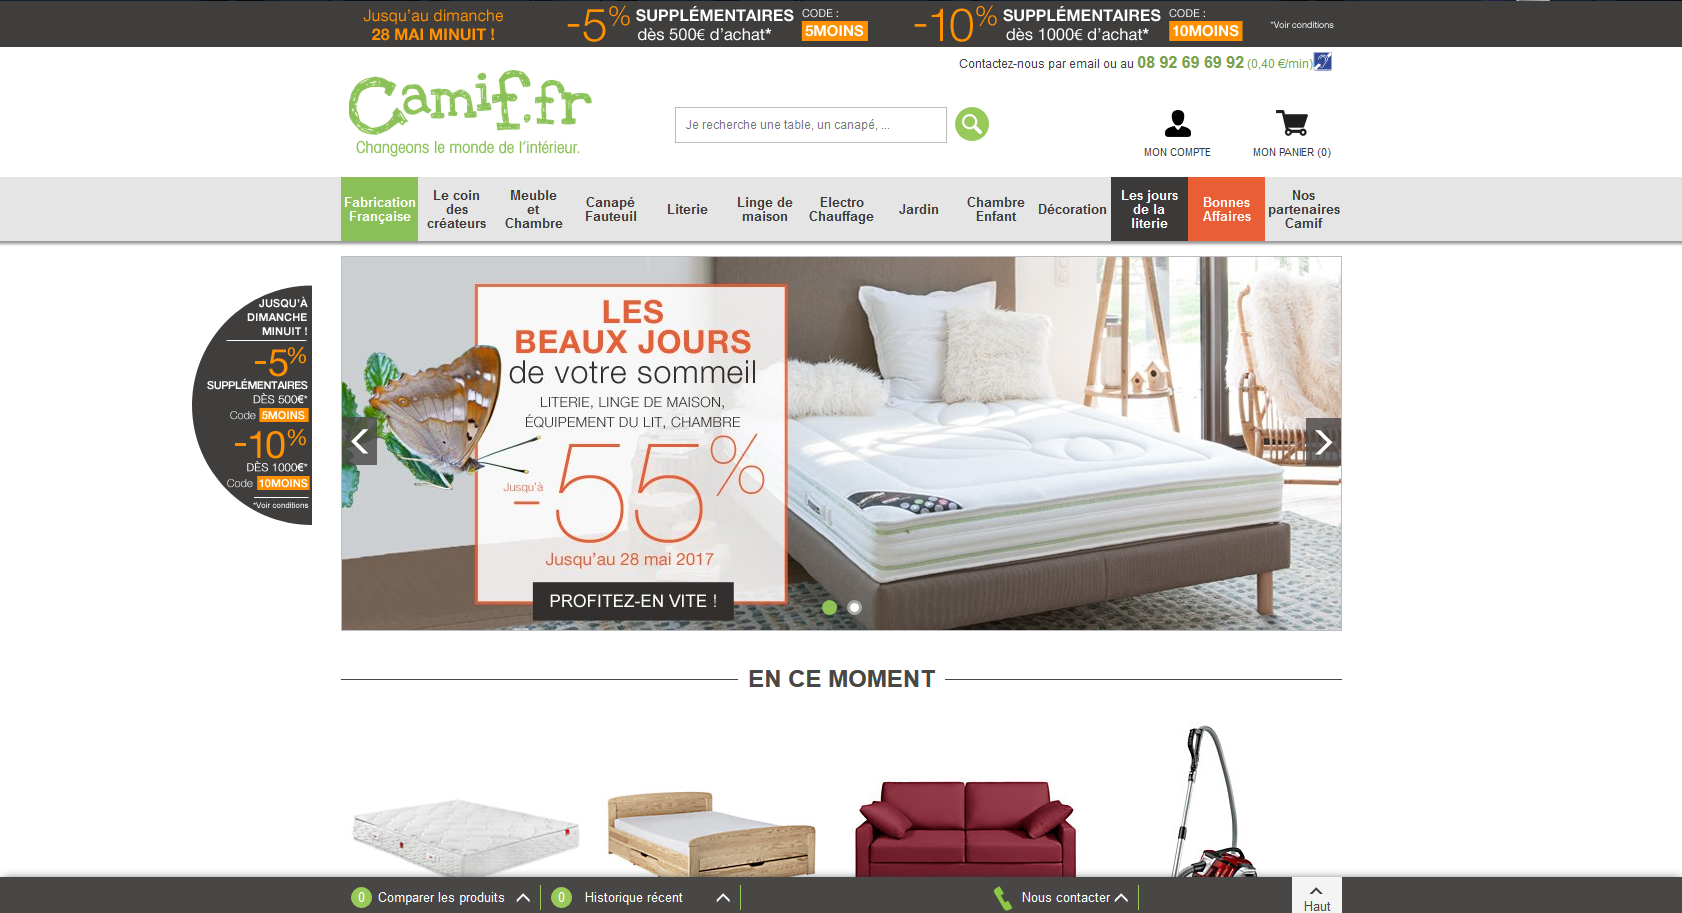
\includegraphics[width=6cm,height=4cm]{Images/CamifPre.PNG}     
	\end{minipage}
	\hfill
	\begin{minipage}[b]{0.45\linewidth}
		\centering
		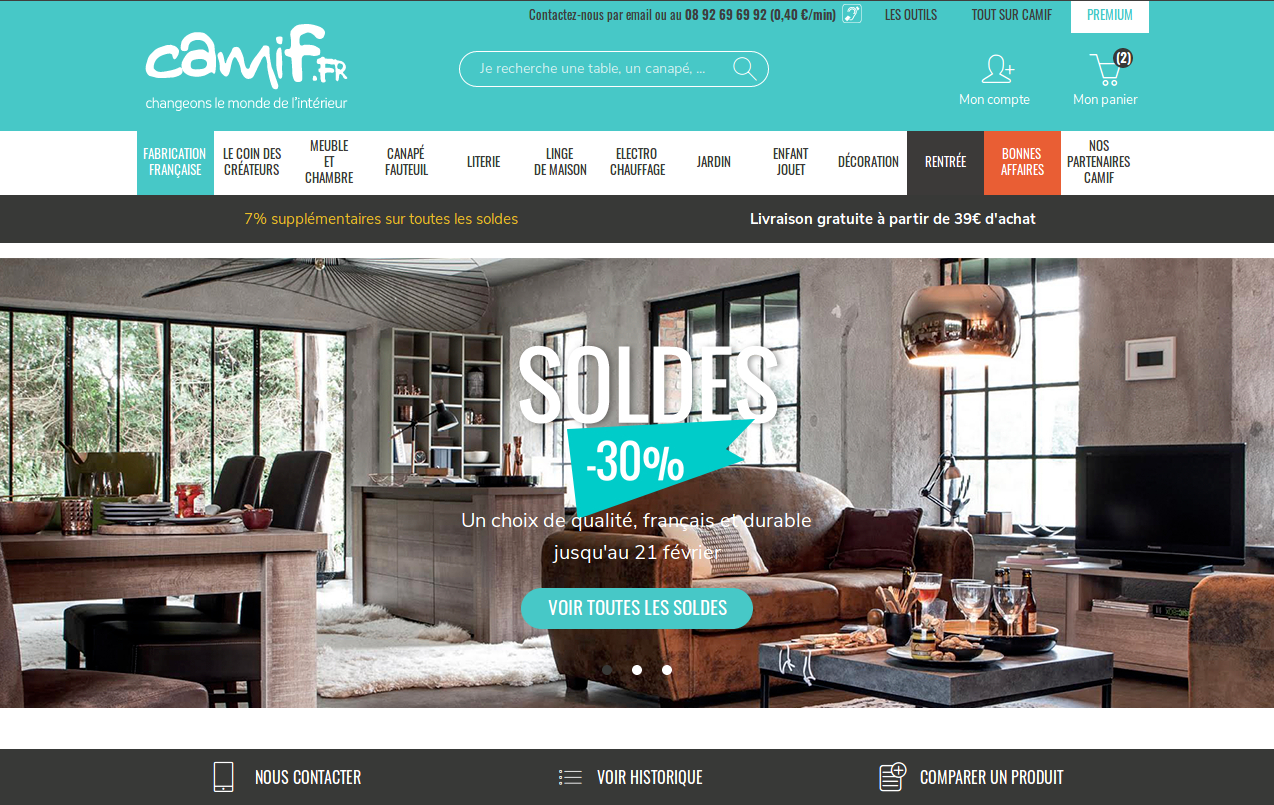
\includegraphics[width=6cm,height=4cm]{Images/CamifPost.png}     
	\end{minipage}
	
	\caption{Refonte du site Camif : à gauche le site actuelle, à droite le site en cours d'évolution}
	
\end{figure}

\subsection{Bocage}

J'ai pris part à ce projet suite à l'absence du développeur initial. Par conséquent, j'ai dû travailler en autonomie et surtout répondre au caractère urgent d'un ticket. Le client a requis la mise en place d'une vidéo dans leur page innovation. Le personnel a tenté d'insérer la vidéo mais cette dernière refusait de se lancer. J'ai donc tout d'abord pris contact avec eux pour connaître leur démarche. Puis avec de la documentation et un brin de patience j'ai pu trouver la cause du problème et le corriger (absence du bloc permettant l'insertion de la vidéo au sein des propriétés XML). \\

Enfin, j'ai eu des difficultés à contribuer à un ticket demandant la suppression des images des catégories sur mobile et non à la dissimuler avec du simple CSS. Le point technique consistait à développer une fonction capable d'identifier si la requête provient d'un mobile. Il existe des solutions open-source capables de le faire mais le but est de ne pas faire grossir l'application pour une seule utilisation. J'ai donc créé une fonction booléenne \texttt{detectHttpMobile()} interrogeant la variable \texttt{\$\_SERVER[...]} et j'ai modifié le \textit{template} pour ajouter la condition et la \textit{Media Query} CSS pour modifier l'apparence de la catégorie selon la taille de l'écran. Enfin, pour vérifier l'efficacité du code, l'application a été testée sur plusieurs appareils mobiles (Android, iOS) via l'outil ngrok.

\subsection{Speed Burger}

Le projet étant à son début de développement et dépendant de la validation des spécifications, j'ai pour mission de créer le formulaire de contact du site. Pour cela, j'ai dû surcharger le formulaire de contact par défaut. Pour pouvoir réaliser les mises à jour de Magento 2 sans difficulté, il est interdit de modifier les fichiers présents dans le dossier \textit{vendor} (code source de Magento). De plus, lorsque que l'on met en place un nouveau module, il est essentiel de penser que le client souhaitera un jour modifier un tel comportement ainsi il faut optimiser le code que pour des actions précises puissent être modifiables dans le \textit{back-office}, par exemple le fait de choisir les e-mails de réception du formulaire. \\

\chapter{Bilan}

Grâce à ce stage j'ai découvert le fonctionnement d'une SS2I. Contrairement à ce que l'on aurait pu penser en écoutant la réputation de certaines entreprises de ce type, mon accueil s'est très bien placé. De plus, afin de faciliter mon intégration au sein d'une équipe et de prendre connaissance des outils de base utilisés chez Smile, j'ai eu la possibilité d'effectuer une formation au sein de leur siège. Cette formation m'a permis de renforcer mes connaissances sur Git et MySQL, de découvrir d'autres outils comme les containeurs LXC ou Ansible et de comprendre l'importance de la gestion des caches. J'ai pu ensuite effectuer une seconde formation sous Magento 2 pour préparer le projet Speed Burger. \\

Grâce aux différents projets auxquels j'ai participé et grâce aux explications et à la patience des équipes, j'ai acquis des notions en gestion de projet et ai pu m'exercer à travailler avec la solution Magento. J'ai également mis en pratique les connaissances acquises lors de ma formation universitaire. \\

Cette expérience, bien que sans lien direct avec la biologie, m'a permis de conforter mon choix de m'orienter dans le développement web. J'espère mettre ces connaissances récemment acquises à profit dans le développement d'une application web dédiée à la biologie.


\mychapter{8}{Webographie}

\begin{itemize}
	\item \textbf{\href{}{stackoverflow.com}} : Stack Overflow est un site d'aide en Informatique en ligne.
	\item \textbf{\href{}{redmine-projets.smile.fr}} : Redmine permet au développeurs de mettre en place un wiki sur un projet et de prendre connaissance des tickets à traiter.
	\item \textbf{\href{}{magento.stackexchange.com}} : Stack Exchange est un site d'aide en ligne spécialisé Magento.
\end{itemize}

\end{document}